%
% File acl2015.tex
%
% Contact: car@ir.hit.edu.cn, gdzhou@suda.edu.cn
%%
%% Based on the style files for ACL-2014, which were, in turn,
%% Based on the style files for ACL-2013, which were, in turn,
%% Based on the style files for ACL-2012, which were, in turn,
%% based on the style files for ACL-2011, which were, in turn, 
%% based on the style files for ACL-2010, which were, in turn, 
%% based on the style files for ACL-IJCNLP-2009, which were, in turn,
%% based on the style files for EACL-2009 and IJCNLP-2008...

%% Based on the style files for EACL 2006 by 
%%e.agirre@ehu.es or Sergi.Balari@uab.es
%% and that of ACL 08 by Joakim Nivre and Noah Smith

\documentclass[11pt]{article}
\usepackage{acl2015}
\usepackage{times}
\usepackage{url}
\usepackage{latexsym}
\usepackage[utf8]{inputenc}
\usepackage{hyperref}
\usepackage[table]{xcolor}
\usepackage{graphicx}
%\setlength\titlebox{5cm}

% You can expand the titlebox if you need extra space
% to show all the authors. Please do not make the titlebox
% smaller than 5cm (the original size); we will check this
% in the camera-ready version and ask you to change it back.


\title{Amazon Web Service vs Google Cloud Plataform}

\author{Author \\
Esperilla Ruiz Adnner,Pacora Jorge \\
  {\tt adnnerer@hotmail.com,JPacora@gmail.com} \\}

\date{}

\begin{document}
\maketitle
\begin{abstract}
    \input{resumen}
\end{abstract}
Amazon Web Service y Google Cloud Plataform ya ha creado una poderosa red global para proporcionar un host virtual para algunos de los entornos de TI más complejos del mundo. Sus centros de datos están conectados por fibra y dispuestos en todo el mundo. En AWS, los pagos se programan de acuerdo exactamente con los servicios que utiliza hasta el milisegundo del tiempo de cómputo. En pocas palabras, tienen una forma rápida y relativamente fácil de migrar sus DevOps a la nube.

\section{Introduction}


\section{Objetivos}
\begin{enumerate}
    \item Son plataformas de servicios de nube que proporciona una variedad de servicios de infraestructura tales como almacenamiento, redes, bases de datos, servicios de aplicaciones, potencia de cómputo, mensajería, inteligencia artificial, servicios móviles, seguridad, identidad y conformidad, entre otros, los cuales permiten el crecimiento de las empresas. 
\end{enumerate}


\section{Marco Teórico}

\subsection{AWS}

\begin{enumerate}
    \item \textbf{AWS CodeBuild:} Este es un servicio de compilación extensible y completamente administrado que proporciona escalado continuo junto con CI y CD. CodeBuild ofrece escalado automático y crece bajo demanda con sus necesidades, por ejemplo, la implementación simultánea de dos versiones de compilación diferentes, lo que permite realizar pruebas de comparación en el entorno de producción. Particularmente importante para muchas organizaciones es la rentabilidad de CodeBuild, porque se le cobra por minuto por los recursos informáticos que utiliza.
    \item \textbf{AWS CodePipeline Crea:} Prueba e implementa su código cada vez que hay un cambio de código, según los modelos de proceso de lanzamiento que defina. Esto le permite ofrecer funciones y actualizaciones de forma rápida y fiable. Puede crear fácilmente una solución de un extremo a otro utilizando los complementos prediseñados para servicios de terceros populares como GitHub o integrando sus propios complementos personalizados en cualquier etapa de su proceso de lanzamiento. Con este CodePipeline, paga por lo que usa, sin tarifas iniciales ni compromisos a largo plazo.
\item \textbf{AWS CodeDeploy:} LCodeDeploy entrega el paquete de trabajo a cada instancia que describe sus parámetros preconfigurados. AWS CodeDeploy automatiza las implementaciones de código en cualquier instancia, incluidas las instancias Amazon EC2 y los servidores locales. AWS CodeDeploy facilita el lanzamiento rápido de nuevas funciones, ayuda a evitar el tiempo de inactividad durante la implementación de la aplicación y maneja la complejidad de actualizar las aplicaciones. Es independiente del código e incorpora fácilmente código heredado común.


\end{enumerate}


\begin{figure}[htb]
\begin{center}
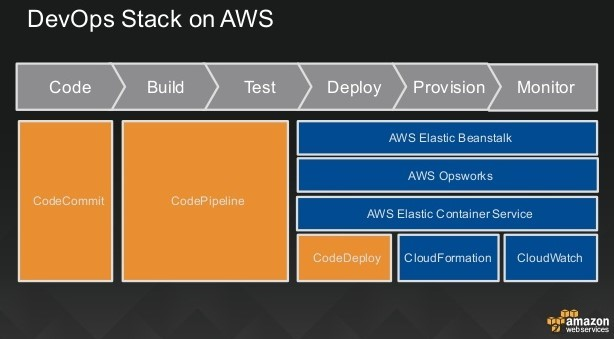
\includegraphics[width=8cm]{./images/imagen1.jpg}
\end{center}
\end{figure}

Además de las herramientas nativas de AWS DevOps, existen algunas opciones de terceros como Chef, Puppet, Jenkins, etc.\\

\subsection{Google Cloud Platform.}
Google Cloud Platform se compone de muchos servicios y soluciones diferentes para utilizar la misma infraestructura de software y hardware que Google usa para sus propios productos (como YouTube y Gmail).\\
Algunos de los principales beneficios de GCP son que es una de las redes de computadoras más grandes y avanzadas, y le brinda acceso a numerosas herramientas para ayudarlo a concentrarse en la construcción de su aplicación. Stackdriver Monitoring, Stackdriver debugger, Stackdriver Logging, servicio de análisis de seguridad (App Engine) y muchos más . Puede usarlos todos inmediatamente como parte de la canalización del ciclo de vida de su aplicación.\\

Las herramientas de administración nativas para el entorno de Google Cloud incluyen los siguientes módulos:\\
\item \textbf{Google Compute Engine:} Google Compute Engine permite a los usuarios lanzar máquinas virtuales bajo demanda. Este es uno de los servicios principales para el aislamiento completo y el escalado automático de instancias únicas a globales. Las VM de Compute Engine se inician rápidamente, vienen con almacenamiento en disco persistente y brindan un rendimiento constante. Sus servidores virtuales están disponibles en muchas configuraciones, incluidos tamaños predefinidos o la opción de crear tipos de máquinas personalizados optimizados para necesidades específicas.\\

Tenga en cuenta que, si compara, Amazon EC2 es esencialmente lo mismo que Google Compute Engine.

\item \textbf{GCP Deployment Manager:} Google Cloud Deployment Manager te permite especificar todos los recursos necesarios para tu aplicación en un formato declarativo usando yaml (o Python, o Jinja2). Esto significa que, en lugar de enumerar minuciosamente cada paso que se requerirá para una implementación, los equipos de DevOps pueden decirle a Deployment Manager cómo debería ser una implementación final y GCP utilizará las herramientas y los procesos necesarios para usted. Cuando se desarrolla un procedimiento de implementación perfecto, se guarda para que sea repetible y escalable a pedido. Con Google Cloud Deployment Manager puedes implementar muchos recursos a la vez, en paralelo, pasar variables a tus plantillas y recuperar los valores de salida, ver tus implementaciones en Google Cloud Console en una vista jerárquica y más.

\item \textbf{GCP Cloud Console:}Cloud Console le brinda una vista detallada de cada detalle de sus DevOps en la nube. Aplicaciones web, análisis de datos, máquinas virtuales, almacén de datos, bases de datos, redes, servicios para desarrolladores ... Google Cloud Console te ayuda a implementar, escalar y diagnosticar problemas de producción en una sencilla interfaz basada en web. Desde máquinas virtuales hasta la administración de versiones y la reversión, domine, supervise y administre todo lo relacionado con GCP desde el escritorio o sobre la marcha. Con GCP Cloud Console para DevOps, puede hacerse cargo fácilmente del ciclo de entrega continua basado en la nube.
\begin{figure}[htb]
\begin{center}
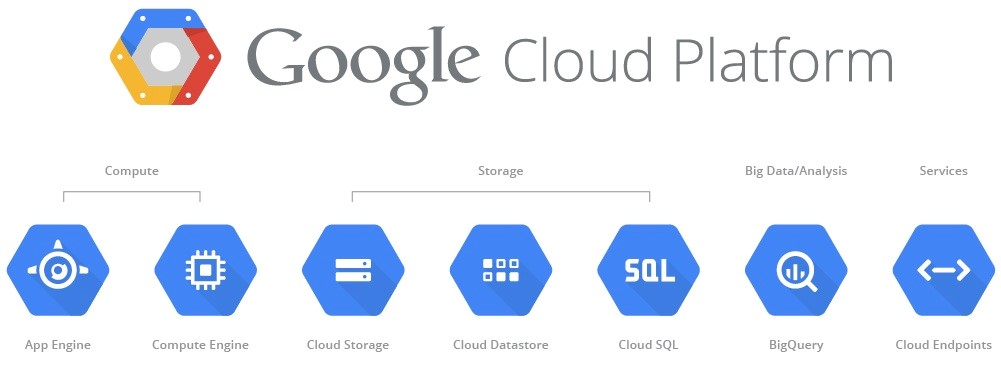
\includegraphics[width=8cm]{./images/imagen2.jpg}
\end{center}
\end{figure}
 \vfill
\section{Tabla comparativa de Google Cloud Platform y AWS}
\endlength
Aqui podremos ver Algunas comparaciones en el siguiente cuadro :
\begin{figure}[htb]
\begin{center}
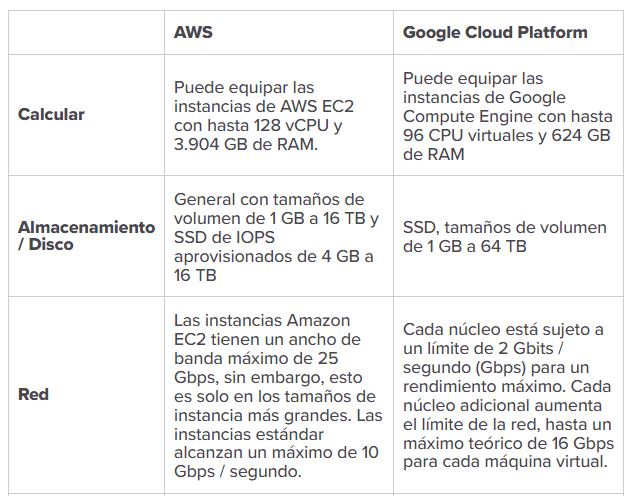
\includegraphics[width=8cm]{./images/imagen3.jpg}
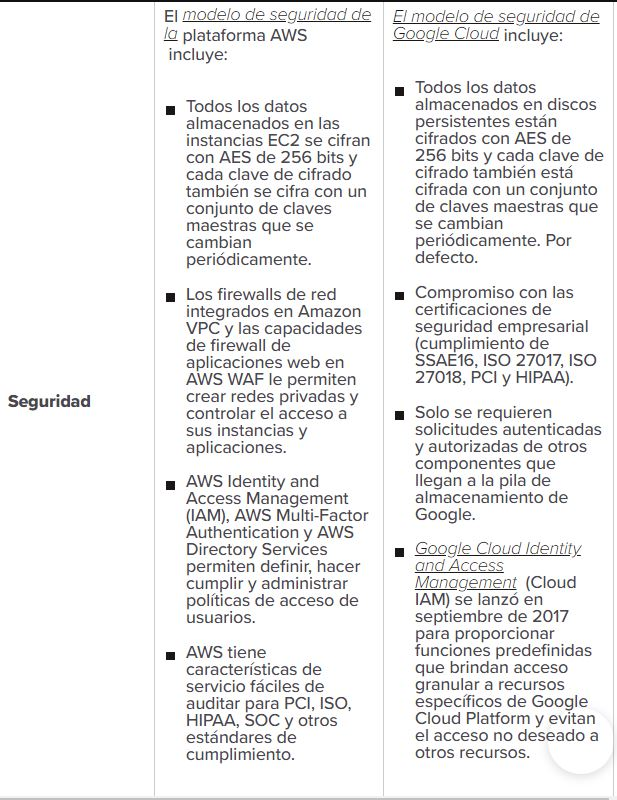
\includegraphics[width=8cm]{./images/imagen4.jpg}
\end{center}
\end{figure}

\section{Conclusiones}

Hoy en día, la computación en la nube se ha vuelto más rentable, confiable y segura. Todos los principales proveedores ahora están invirtiendo en su hardware, software e infraestructura de red global para obtener más participación de mercado. Debido a la competencia entre ellos, los equipos de DevOps recibieron soluciones muy sofisticadas, fáciles de integrar, rápidas y de alta gama. Como la calidad sigue siendo casi igual, la diferencia entre los principales proveedores de computación en la nube radica principalmente en el precio y la cantidad de opciones que obtiene.

Lo que también puede marcar la diferencia son las zonas de operación. AWS opera 49 zonas de disponibilidad dentro de 18 regiones geográficas, con planes anunciados para 12 zonas de disponibilidad más y cuatro regiones más en Bahrein, Hong Kong SAR, Suecia y una segunda región de AWS GovCloud en los EE. UU. Mientras que Google Cloud Platform tiene 13 regiones, 39 zonas, más de 100 puntos de presencia y una red global con 100,000 millas de cable de fibra óptica.

Teniendo en cuenta una participación de mercado, AWS es líder. Google está haciendo un buen progreso, pero tiene mucho más trabajo por hacer para demostrar que es una opción empresarial viable.

AWS es líder en términos de número de clientes y productos. Por otro lado, GCP ya proporciona toda la funcionalidad necesaria y ofrece buenos precios junto con modelos de configuración, respaldados por serias medidas de seguridad y privacidad del tráfico.

Entonces, ¿qué es mejor para DevOps en la nube? Como es habitual, no damos respuesta pero te mostramos las alternativas para elegir. Ahora, cuando tenga todos los datos, tendrá el poder de tomar sus propias decisiones para su equipo de DevOps.

% include your own bib file like this:
%\bibliographystyle{acl}
%\bibliography{acl2015}


\begin{thebibliography}{9}
    \bibitem{The DevOps Handbook Gene Kim} 
    churriwifi
    \textit{https://www.amazon.com/DevOps-Handbook-World-Class-Reliability-Organizations/dp/1942788002/ref=sr_1_3?ie=UTF8&qid=1529684136&sr=8-3&keywords=devops+handbookl/}. 
    

    \bibitem{Accelerate: The Science of Lean Software and DevOps: Building and Scaling High Performing Technology Organizations Nicole Forsgren ,Patrick Deboys} 
    bi-geek\\
    \textit{https://www.amazon.com/Accelerate-Software-Performing-Technology-Organizations/dp/1942788339/ref=sr_1_13?dchild=1&keywords=devops&qid=1598217512&sr=8-13/}
    
    
    
    


\end{thebibliography}


\end{document}